\section{Scenarios and Results}
In order to test the simulation framework, three different scenarios were created with unique design choices and characteristics. Each of them designed to represent a simplified real-world scenario with their own challenges and management implications. These scenarios represent three major types of fires: Extreme weather events, human-wildland interface conditions and complex coastal fire dynamics. Each of the scenarios have different parameter sets and environmental conditions to show the models ability to capture a diverse fire behaviors.

\subsection{Drought Firestorm Scenario}
The first scenario represents a very extreme fire weather conditions and intends to simulate the type of catastrophic fires that occur after a long period drought with very low level of moisture. These types of conditions are becoming more prevalent with the climate change, that we are experiencing right now. Furthermore this scenario serves as baseline for maximum fire potential and validates the model ability to handle a large number of fire events similar to California's recent Megafires or Australia's Black Summer fires.
\subsubsection{Configuration Parameters}
Environmental Setup:
\begin{itemize}
	\item \textit{Map Type}: Forest terrain with homogeneous fuel distribution
	\item \textit{Wind conditions}: 0 (still air conditions)
	\item \textit{Grid Dimensions}: 100 $\times$ 100 cells
	\item \textit{Moisture}: 0 (drought conditions)
	\item \textit{Fuel Types}: 6 distinct heterogeneous patches
	\item \textMultiple ignition points
\end{itemize}
Key Fire Behavior Parameters:
\begin{itemize}
	\item \texttt{spread\_rate}: 0.08 (base velocity of particles, high spread potential)
	\item \texttt{ignition\_probability}: 0.15 (base probability for ignition)
	\item \texttt{particle\_generation\_rate}: 0.18 ( rapid fire particle production))
	\item \texttt{burnout\_rate}: 0.005 (Rate at which burning cells burnout)
\end{itemize}
\begin{figure}[H]
	\centering
	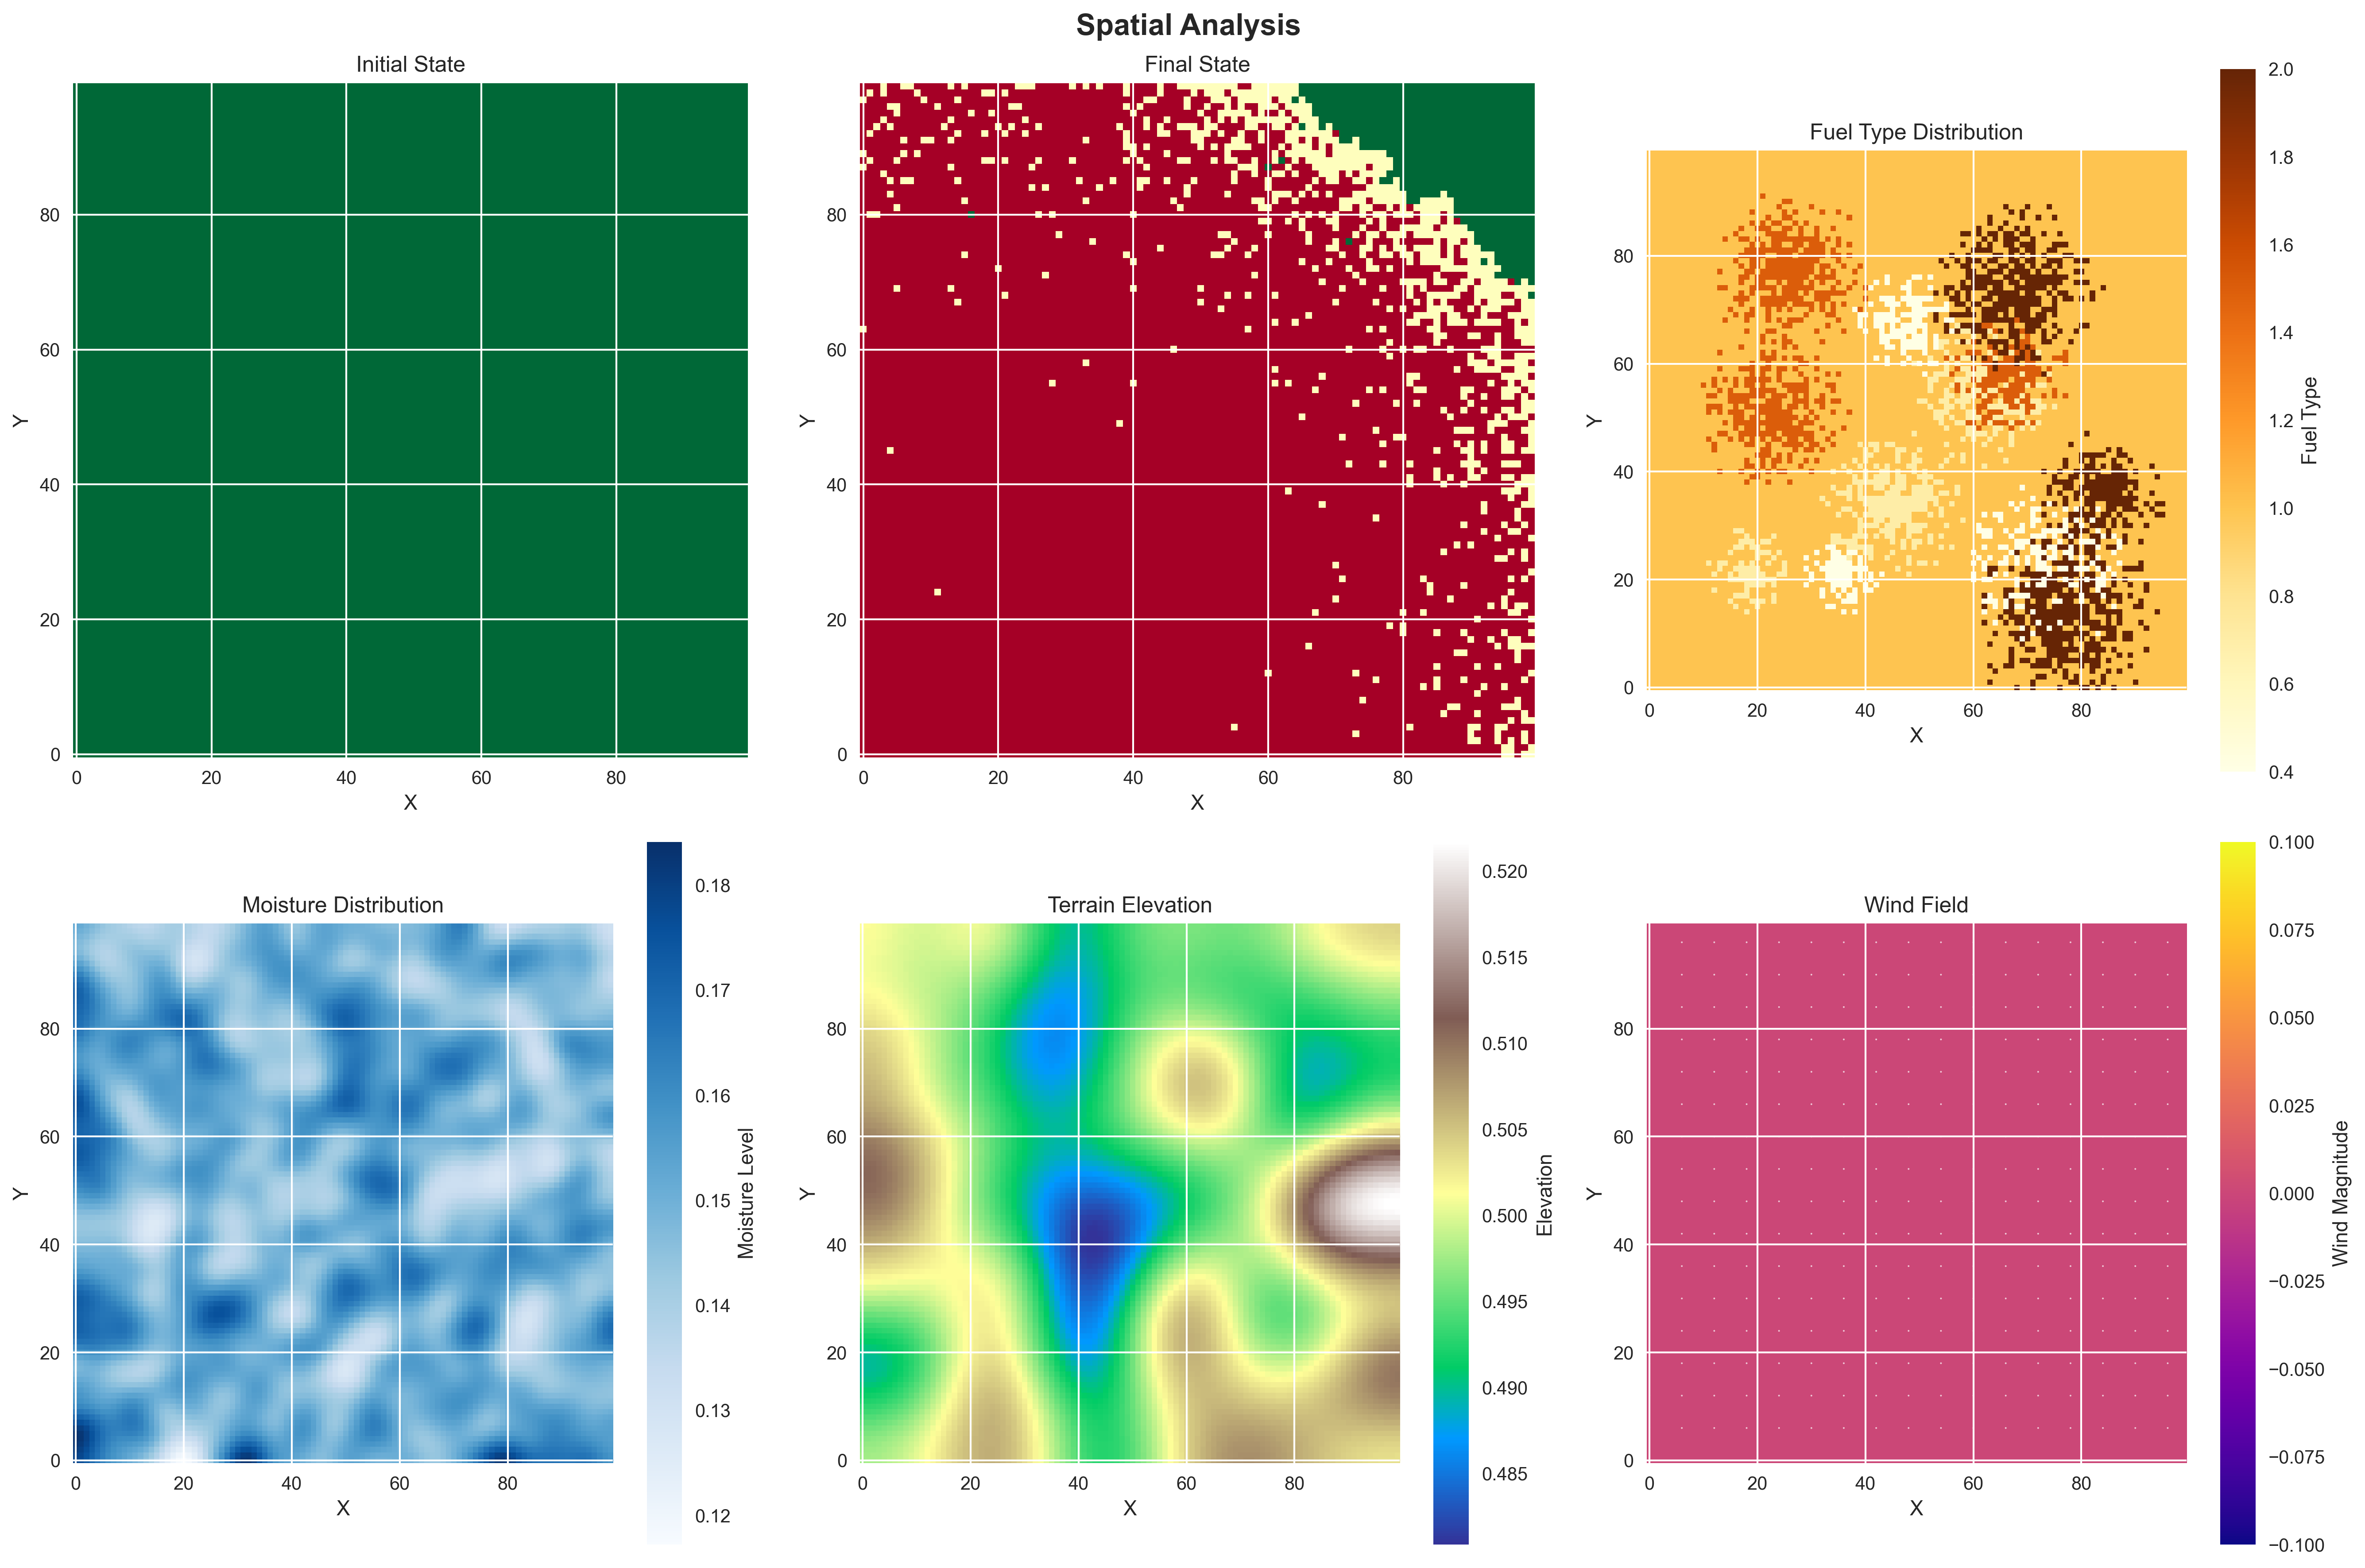
\includegraphics[width=\textwidth]{media/spatial_analysis_df.png}
	\caption{
		\textbf{Spatial Analysis - Drought Firestorm Scenario.}
		Environmental conditions and fuel distribution for the drought firestorm simulation. Top row shows initial state (left) with uniform fuel distribution, final state (center) with extensive burned area coverage, and fuel type distribution (right) with heterogeneous patches ranging from grassland (light) to dry brush (dark). Bottom row displays moisture distribution (left) showing minimal moisture content, terrain elevation (center) with topographic variations, and wind field (right) showing on wind.
	}
	\label{fig:spatial_df}
\end{figure}

\subsubsection{Fire Progression Analysis}
Figure~\ref{fig:spatial_df} shows the spatial analysis of the simulation, which reveals several patterns.
Initially the simulation begins with a uniform fuel distribution across the entire grid, with fuel values ranging from 0.4 to 2.0. It also presents an absence of moisture or empty cells, which acts as boundaries in the simulation. These conditions create a scenario, where the fire spreads unrestrictedly. Looking at the fire progression dynamics in Figure~\ref{fig:res_df} we can observe the following in different stages:
\begin{itemize}
	\item \textbf{Early Stage (Frames 10)}: Initial multiple ignition points, which ignite the forest fire at multiple points (shown in dark green). The fire starts spreading in a radial pattern from each ignition point.
	\item \textbf{Mid Stage (Frame 760)}: By this point the fire has spread aggressively and merged into a one single fire front. This culminates in over 1000 particles at around the 1000th frame and the peak fire intensity.
	\item \textbf{Final Stage (Frame 1500)}: Roughly 85\% of the total area is burned and due to the limited amount of fuel remaining the fire intensity declines.
\end{itemize}

\subsubsection{Quantitative Fire Dynamics}
When looking at the Cell State Evolution in Plot A, the progression over time show a classic wildfire behavior, where the fuel is steadily decreasing while the burned cells are increasing. The Burning cells, show an initial strong incline caused by the ignition, followed by a roughly constant number of burning cells, finally when the fuel diminishes, so does the number of burning cells. Plot B and C shows a similar picture, where initially the burned state show a slow spread, which then rapidly increases and the decelerates when the fuel becomes sparse. Plot C also highlights the interplay between the burned cells and the number of particles, where at the beginning the large number of particles create by the ignition, increases the burning cells and the afterwards the decreasing number of burning cells causes the generation of particles to stop and the missing flue causes the number of particles to decrease.\newline
\newline
Looking at the fire intensity, the burn rate peaks at 16.0 cells per frame with an average burn rate of 5.67. Furthermore the distribution resembles a bell curve with a peak intensity between 600 and 1000 frames. The fire spread velocity shows a maximum spread rate of 0.95 units per frame with a high variability during active burn phases. Similar to the other plots the decrease of particles shows a clear reduction in velocity as fire approach the fuel boundaries.\newline
\newline
Despite zero wind conditions, the drought simulation showed a realistic fire spread patterns driven by:
\begin{itemize}
	\item Fuel heterogeneity effects, driven by different types of fuel creating a preferential spread pathways
	\item Terrain Influences, where slop effects affected spread.
	\item Particle dynamics, where stochastic particle movement created irregular fire perimeters.
\end{itemize}
\begin{figure}[H]
	\centering
	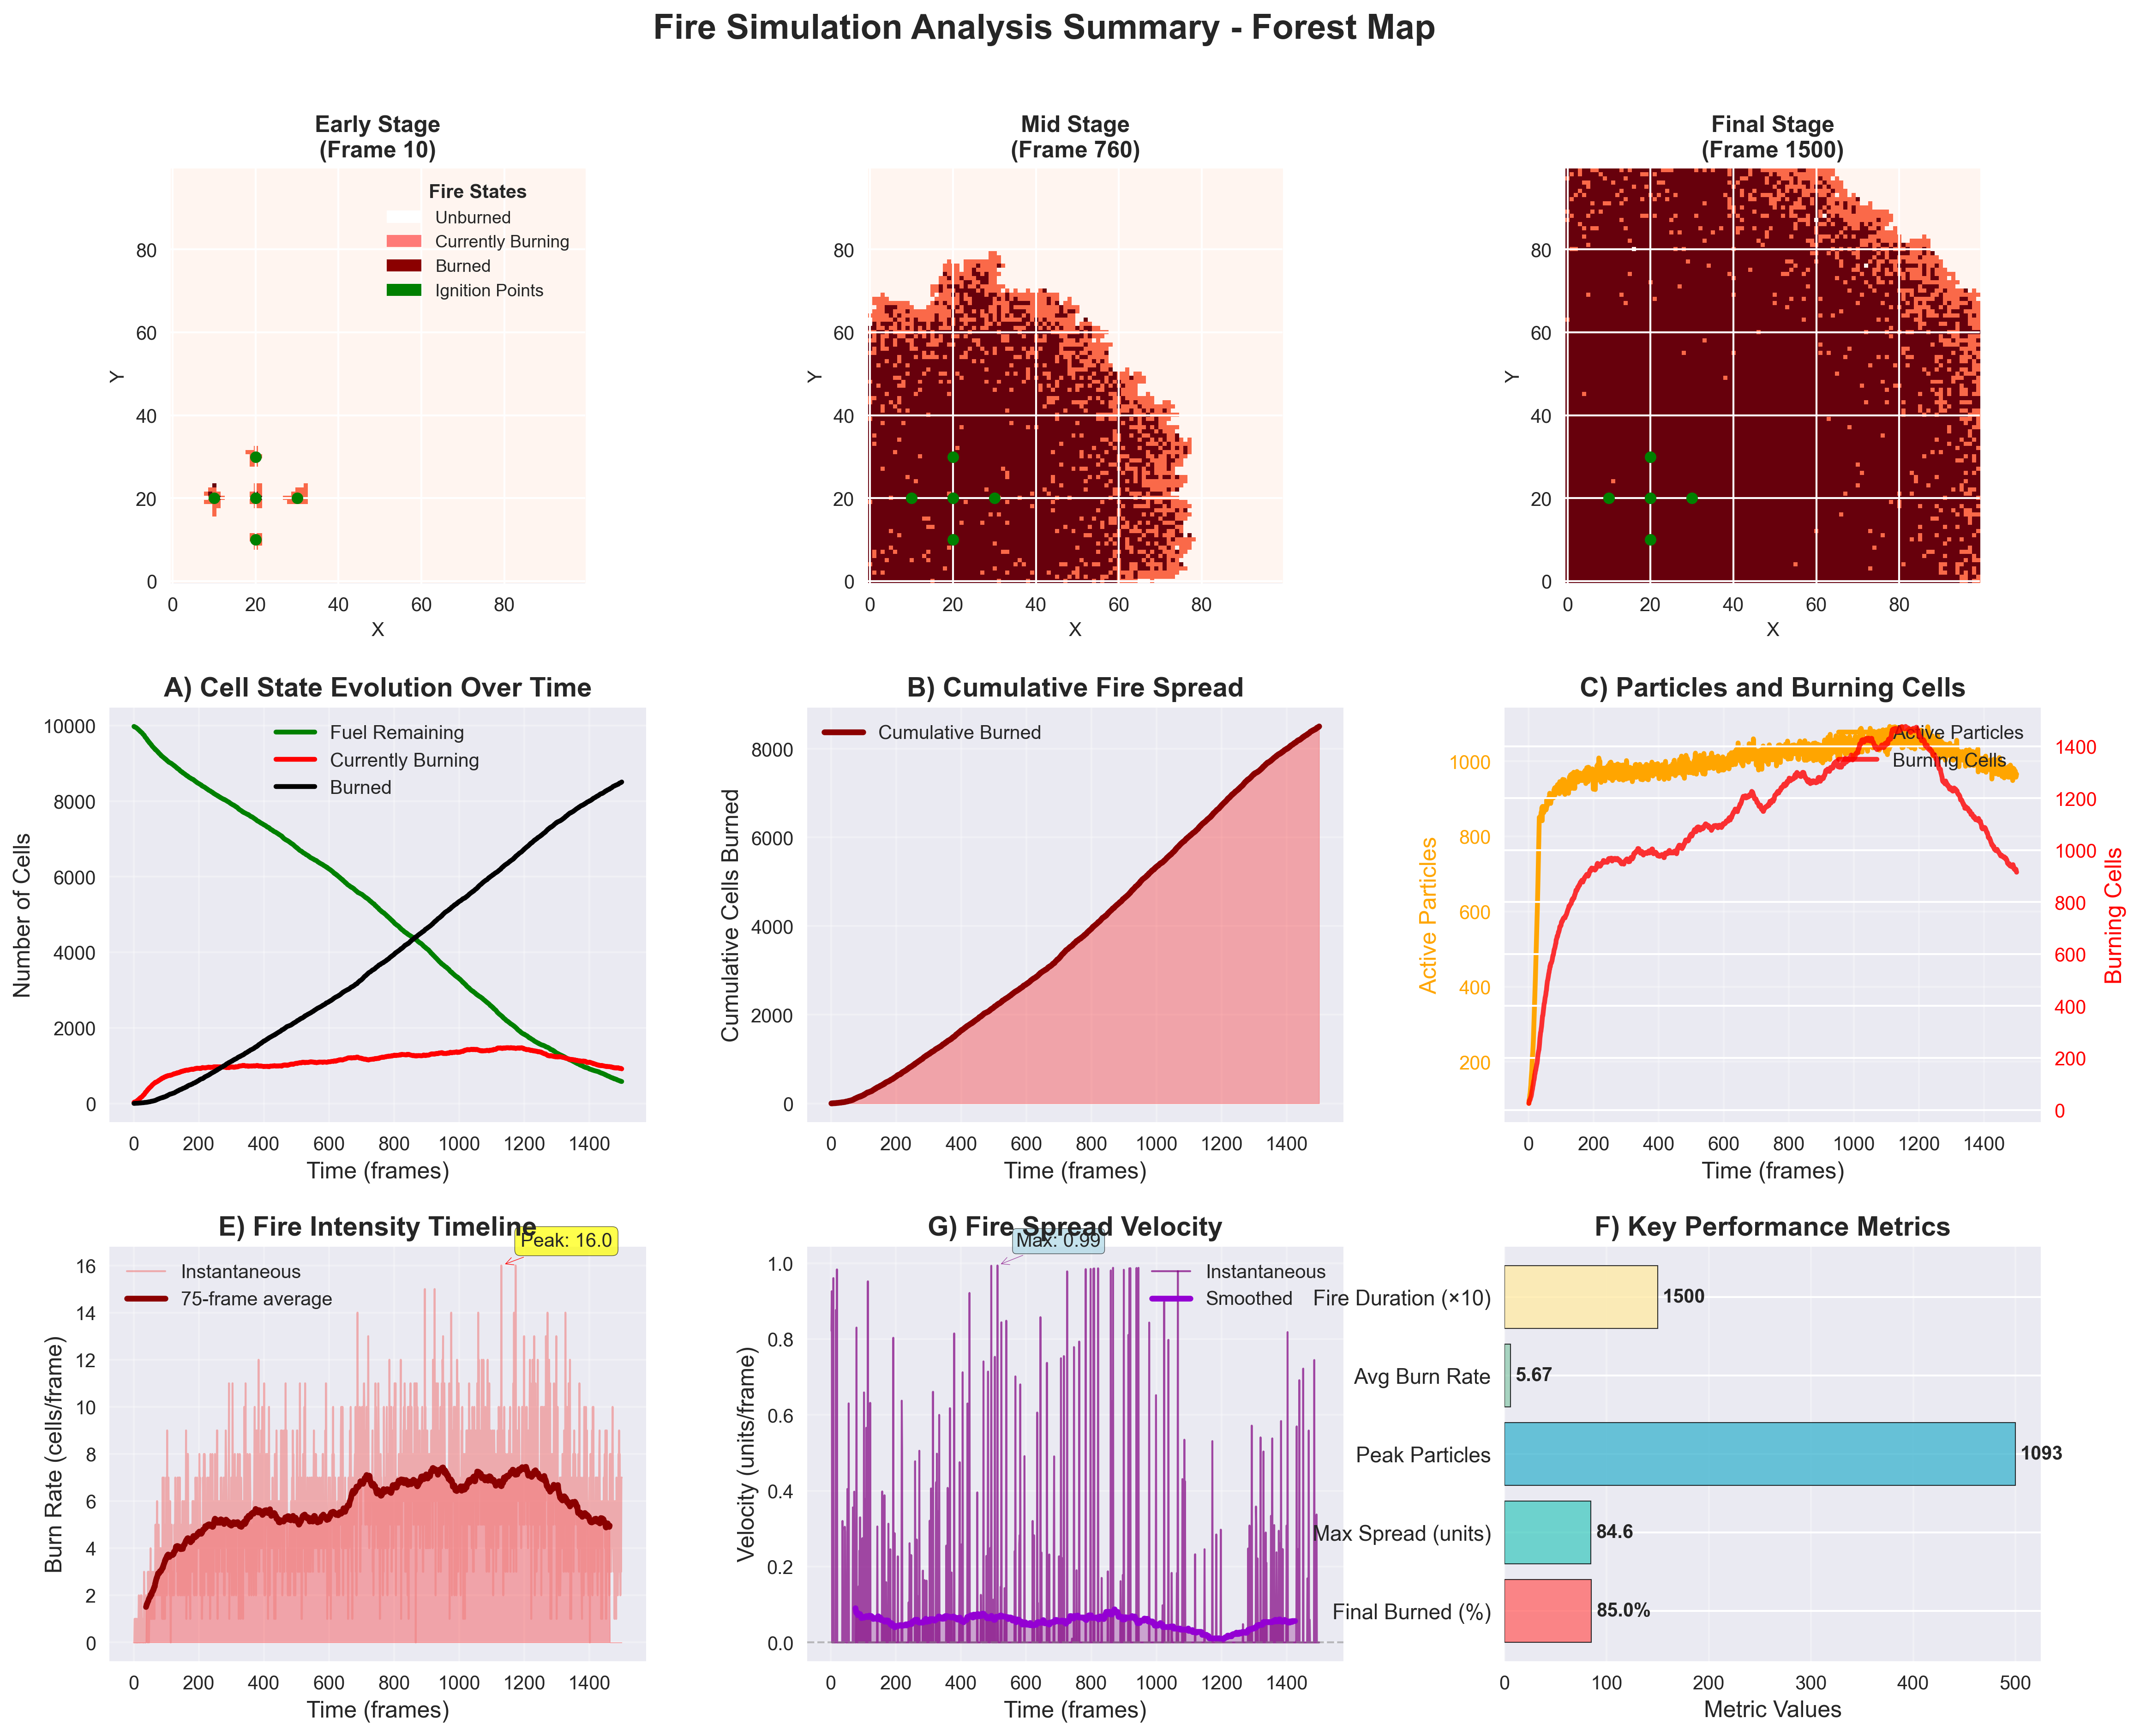
\includegraphics[width=\textwidth]{media/report_summary_df.png}
	\caption{
		\textbf{Fire Simulation Analysis Summary - Drought Firestorm.}
		Comprehensive analysis of fire progression under extreme drought conditions. Top row shows fire evolution from early ignition (left) through mid-stage development (center) to final extensive coverage (right). Middle row presents cell state evolution over time (A), cumulative fire spread (B), and particle-burning cell dynamics (C). Bottom row displays fire intensity timeline (E), fire spread velocity (G), and key performance metrics (F) including 85.9\% final burned area and peak particle count of 1093.
	}
	\label{fig:res_df}
\end{figure}

\subsection{Wildland Urban Scenario}
The second scenario is dedicated to a wildland-urban interface scenario and intended to address one of the most challenging in modern fire management, which is protecting residential communities located within or close to wildland areas. This scenario becomes increasingly relevant with urban expansion into fire-prone landscapes.
\subsubsection{Configuration Parameters}
Environmental Setup:
\begin{itemize}
	\item \textit{Map Type}: WUI with scattered housing clusters
	\item \textit{Wind}: Moderate with directional bias (strength $=0.6$, direction $=0.75 \pi$)
	\item \textit{Moisture}: Low with defensive space around the buildings
	\item Structures create firebreaks and modify local moisture
\end{itemize}
Fire Behavior Parameters:
\begin{itemize}
	\item \texttt{spread\_rate}: 0.06 (moderate spread potential)
	\item \texttt{ignition\_probability}: 0.12 (reduced due to fuel treatments)
	\item \texttt{intensity\_decay}: 0.98 (faster intensity decay than wildland)
	\item \texttt{particle\_lifetime}: 20 (extended for spot fire modeling)
\end{itemize}
\begin{figure}[H]
	\centering
	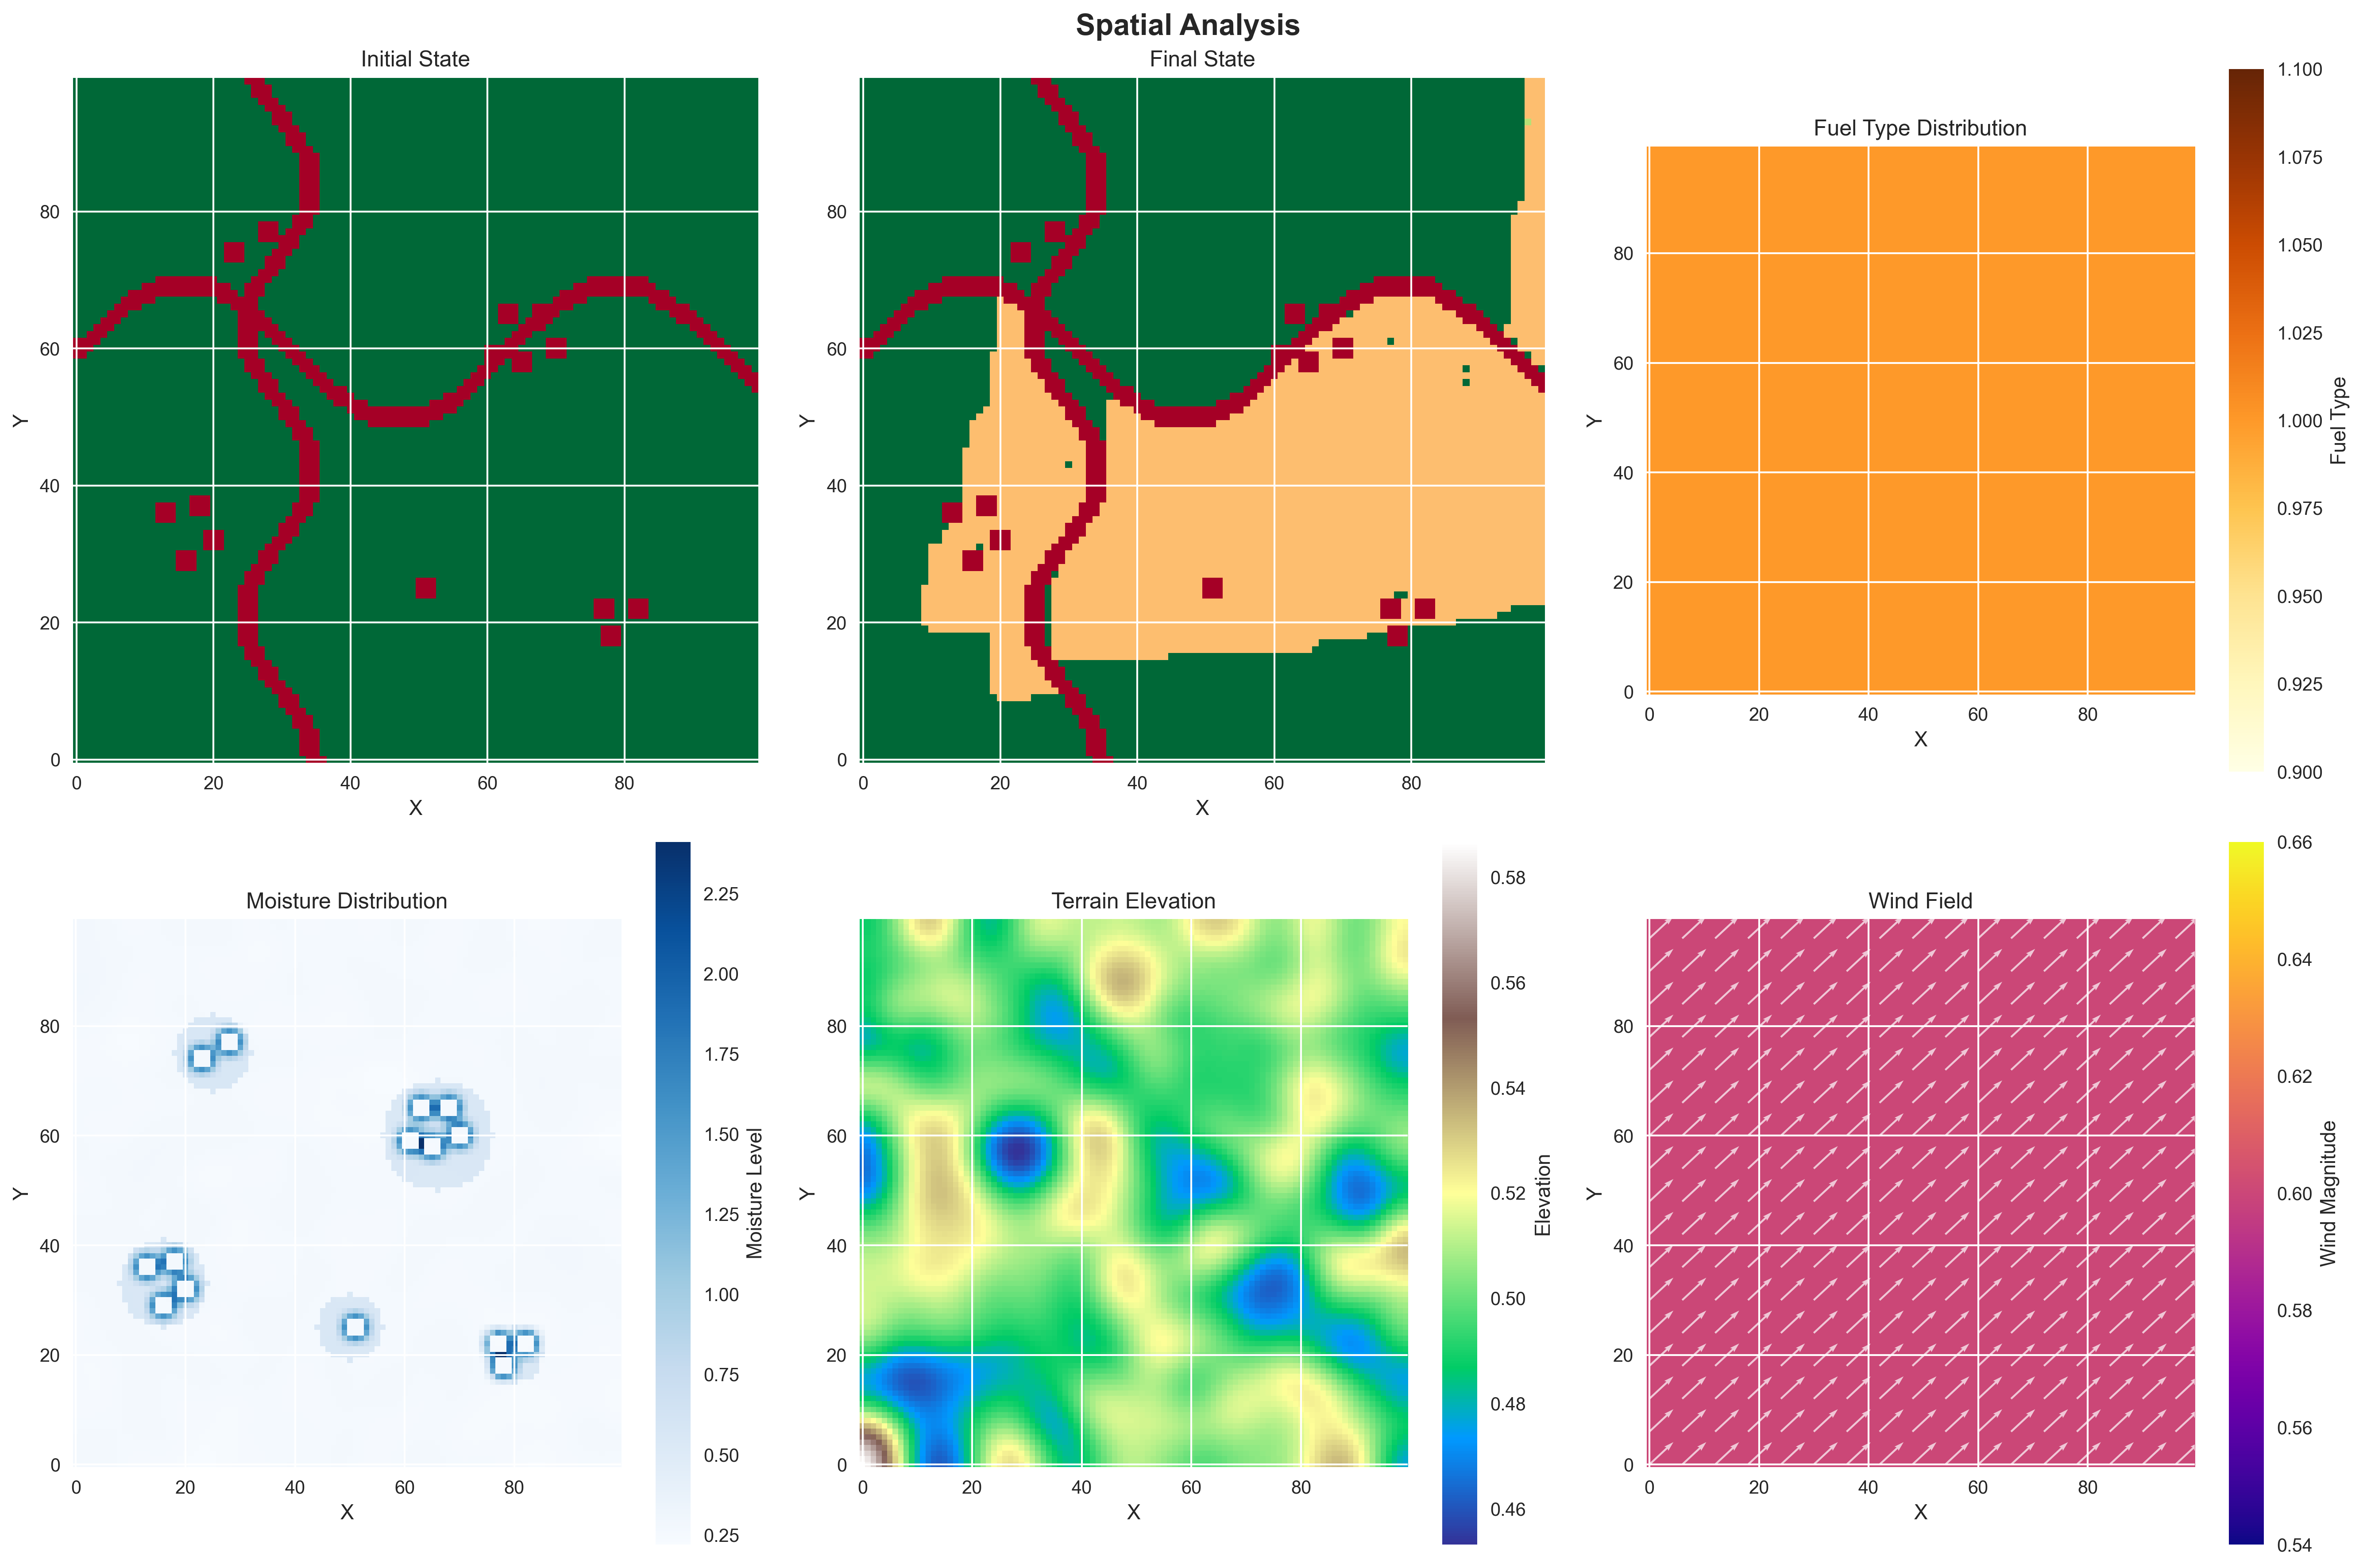
\includegraphics[width=\textwidth]{media/spatial_analysis_wui.png}
	\caption{
		\textbf{Spatial Analysis - Wildland Urban Interface Scenario.}
		Environmental conditions for WUI fire simulation showing the interaction between natural fuels and residential development. Top row displays initial state (left) with scattered housing clusters and defensible space, final state (center) showing fire containment around structures, and fuel type distribution (right). Bottom row shows moisture distribution (left) with elevated moisture around structures, terrain elevation (center), and wind field (right) with moderate directional wind creating asymmetric fire spread potential.
	}
	\label{fig:spatial_wui}
\end{figure}

\subsubsection{Fire Progression and Structure Protection}
Figure~\ref{fig:spatial_wui} shows the environmental conditions for the WUI fire simulation, with afford mentioned housing clusters with a base moisture level of 0.1, which increased to 0.4-0.7 around the houses.\newline
If we analyse the fire progression seen in Figure~\ref{fig:res_wui} we can observer the following about the Stages:
\begin{itemize}
	\item \textbf{Early Stage (Frames 10)}: Multiple Ignition points strategically placed on either side of the vertical river. The fire starts to spread not in a radial pattern this time due to the wind.
	\item \textbf{Mid Stage (Frame 760)}: By this point the fire has expanded significantly. This includes around the housing structures, the simulation also show that it took longer to burn the are behind a house due to the wind, but the fire was still able to reach those areas. Furthermore the rivers acted like a barrier and fire was not able to jump across except on the thinnest part of the horizontal river on the right side.
	\item \textbf{Final Stage (Frame 1500)}: Roughly 35\% of the total area was burned, which preserved substantial amount of fuel and the rivers acted as a successful barrier to contain the fire. Also the wind had a clear influence that the fire was pushed into the wind direction, leaving substantial fuel patches in this case on the bottom and left part of the map untouched.
\end{itemize}
\begin{figure}[H]
	\centering
	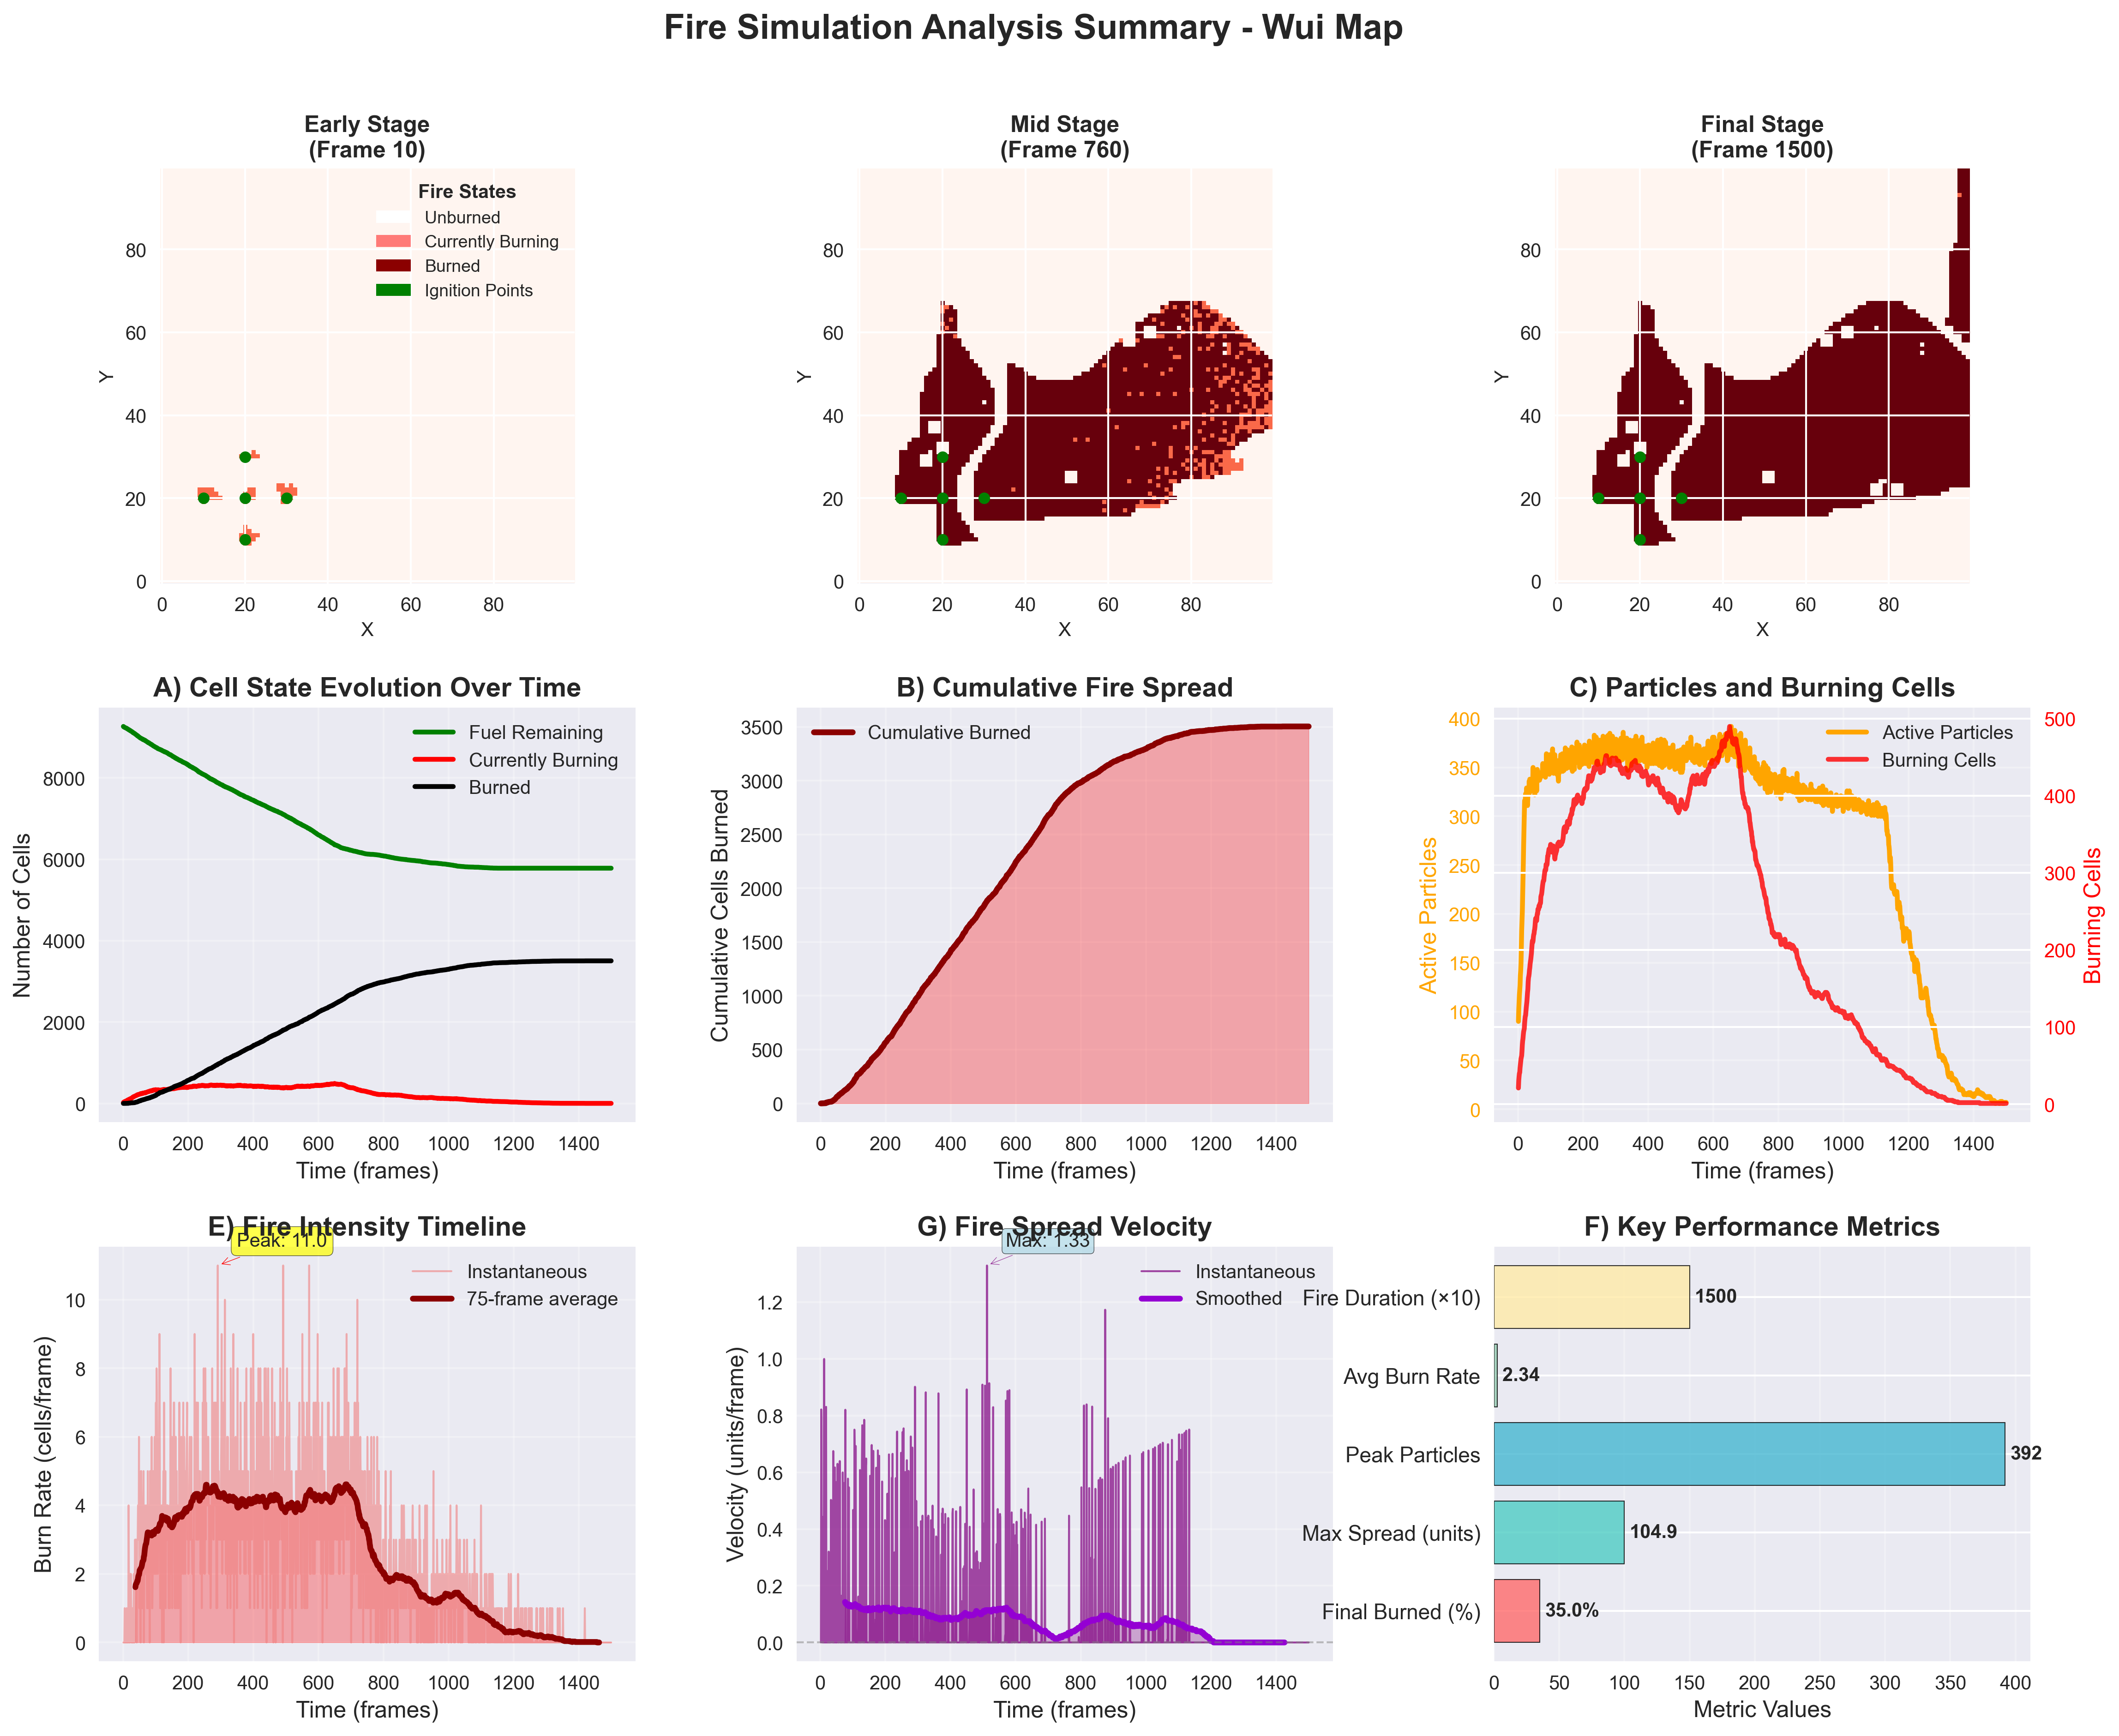
\includegraphics[width=\textwidth]{media/report_summary_wui.png}
	\caption{
		\textbf{Fire Simulation Analysis Summary - Wildland Urban Interface.}
		Analysis of fire behavior in developed wildland areas demonstrating effective structure protection. Top row shows fire progression with early containment (left), mid-stage development around barriers (center), and final controlled burn area (right). Middle and bottom rows present temporal analysis showing reduced fire intensity compared to drought conditions, with 35.0\% final burned area and successful defensible space performance protecting all residential structures.
	}
	\label{fig:res_wui}
\end{figure}
\subsubsection{Quantitative Fire Dynamics}
The quantitative fire dynamics data shown in graphs A, B and C demonstrated the controlled fire behavior with initial incline in burned cells and then a gradual decline. The fire reach its peak at around 600 time frames. Especially Plot C shows significant decline of number of burning cells, which is then followed with a delay by the number of particles. A similar pattern can be observed, when looking at the fire intensity timeline Plot E, where the intensity peak was reached rather early at 11.0 burning cells per frame.\newline
\newline
Lastly looking at the fire intensity we can can observe the high fluctuations reflecting encounters with fuel patches and barriers. We can also clearly observe the spot where the fire spread over to the other side of the river around the 700 time frame mark.\newline
\newline
In conclusion this scenario demonstrated the effectiveness of obstacles to reduce fire spread, but still showed that the fire can wrap around houses with not enough protection. It also clearly shows the immense impact that wind strength and direction has on a wildfire situation.

\subsection{Coastal Scenario}
The coastal scenario is a complex fire dynamics found in ,for example Mediterranean, coastal regions, where strong offshore winds interact with the natural moisture gradient and varied vegetation types. This coastal environment present a unique challenge due to the interaction between maritime influences, such as high moisture near the coast and continental effects, such as dry condition inland, combined with a topographic complexity and a strong and variable wind blowing land inwards. This scenario intends to test the model's ability to simulate gradient effects and wind-driven fire behavior.
\subsubsection{Configuration Parameters}
\textbf{Configuration}
\begin{itemize}
	\item \textit{Map Type}: Coastal with moisture gradient
	\item \textit{Wind}: Strong offshore winds
	\item \textit{Moisture}: Gradient from high coastal (0.4) to low inland (0.1)
	\item Variable wind patterns simulating sea/land breeze
\end{itemize}
\textbf{Key Parameters:}
\begin{itemize}
	\item \texttt{spread\_rate}: 0.10
	\item \texttt{ignition\_probability}: 0.18
	\item \texttt{intensity\_decay}: 0.94
	\item \texttt{particle\_lifetime}: 22
	\item \texttt{burnout\_rate: 0.03}
\end{itemize}
\subsubsection{Coastal Fire Progression}
The Scenario employs multiple ignition points at different distances from the coast, with the intention of having ignition points at the different levels of fuel types, which are layered in such a way that you have three different zones:
\begin{itemize}
	\item \textit{Near-coast zone}: High moisture and low flammable fuel.
	\item \textit{Transition zone}: Moderate fire spread
	\item \textit{Inland zone}: More aggressive fire behavior
\end{itemize}
Furthermore we a wind-driven inland penetration, due to strong offshore winds drive the particle inland, creating a characteristic fire behavior.
\begin{itemize}
	\item \textbf{Early Stage (Frames 10)}: The six ignition are ignite in the different zones and we can already see how the wind blows the particles inland.
	\item \textbf{Mid Stage (Frame 760)}: The fire was able to jump over into other zones, furthermore it is clearly visible that fire struggled to burn in zones closer to the coast and only the inland fires are still active at this point.
	\item \textbf{Final Stage (Frame 1500)}: The fire has further expanded inland and is still burning up the remaining high fuel areas.
\end{itemize}
\begin{figure}[H]
	\centering
	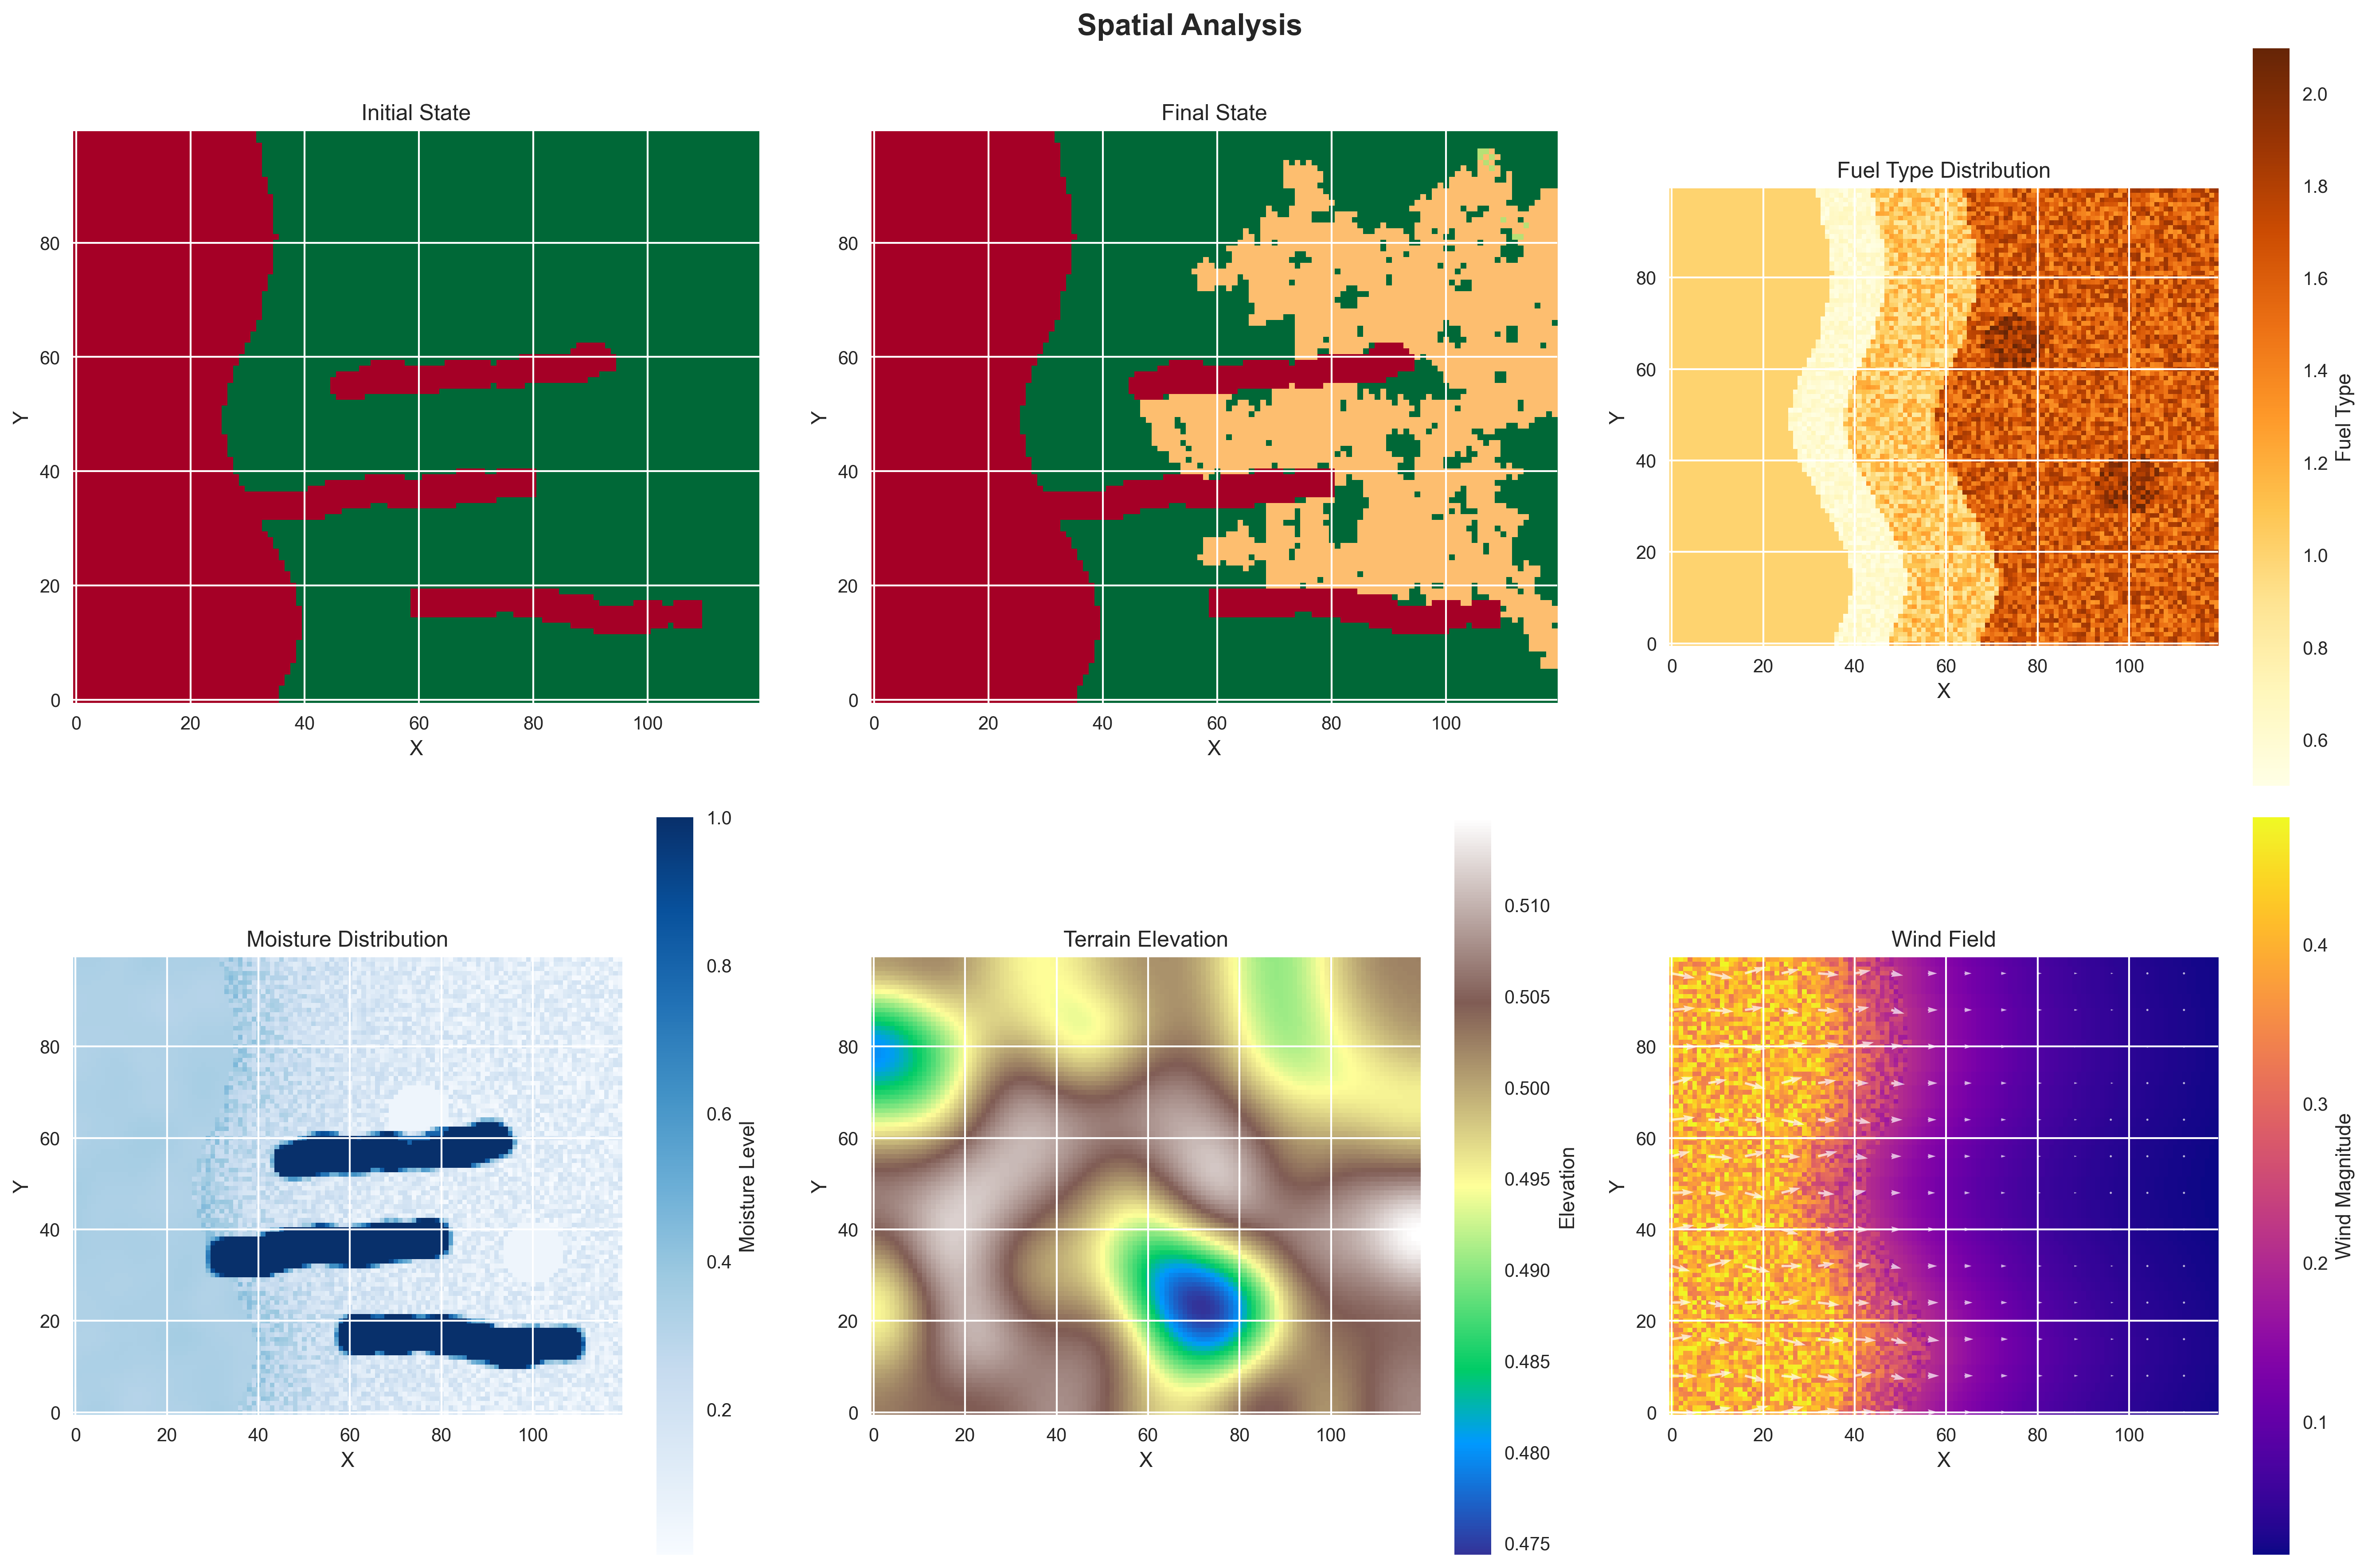
\includegraphics[width=\textwidth]{media/spatial_analysis_coast.png}
	\caption{
		\textbf{Spatial Analysis - Coastal Fire Scenario.}
		Environmental conditions for coastal fire simulation featuring moisture gradients and strong offshore winds. Top row shows initial state (left) with coastline and natural barriers, final state (center) demonstrating inland fire penetration with coastal protection, and fuel type distribution (right) varying from coastal scrub to inland chaparral. Bottom row displays moisture distribution (left) with clear coastal-to-inland gradient, terrain elevation (center), and strong wind field (right) creating offshore wind patterns typical of extreme fire weather events.
	}
	\label{fig:spatial_coast}
\end{figure}
\subsubsection{Quantitative Fire Dynamics}
The quantitative fire dynamics data presented in graphs A, B and C of Figure~\ref{fig:res_coast} showed controlled fire behavior characteristic of coastal environments. The cell state evolution (Plot A) shows gradual fuel depletion with a double-peaked pattern around frames 400 and 800, indicating episodic fire activity as the fire reaches alternating moisture zones. The cumulative fire spread (Plot B) has three distinct phases: a slow coastal suppression, moderate inland acceleration, and final plateau at 28.4\% burned area, which is the lowest among all scenarios. \newline
\newline
Graph C reveals the interaction between active particles and burning cells, where the particles leading ignition events by roughly 50 frames. The fire intensity timeline (Plot E) shows sustained moderate activity with high temporal variability and peak intensity of 8.0 cells per frame, which is lower by a large margin compared to the drought conditions.\newline
\newline
The fire spread velocity (G) shows extreme fluctuations, which is characteristic for a scenario which includes a lot of barriers. The maximum sustained velocity ( 0.6 units per frame) happens during coastal barrier breakthrough events. This clear velocity spikes correspond to the fire extending through zone barriers and entry into drier inland fuel zones.\newline
\newline
In conclusion, this scenario demonstrated the effectiveness of natural moisture gradients in fire suppression, achieving 57.5\% reduction in burned area compared to drought conditions. The coastal barriers successfully contained  fire spread while strong offshore winds were driving the particles in a predictable directional inland.
\begin{figure}[H]
	\centering
	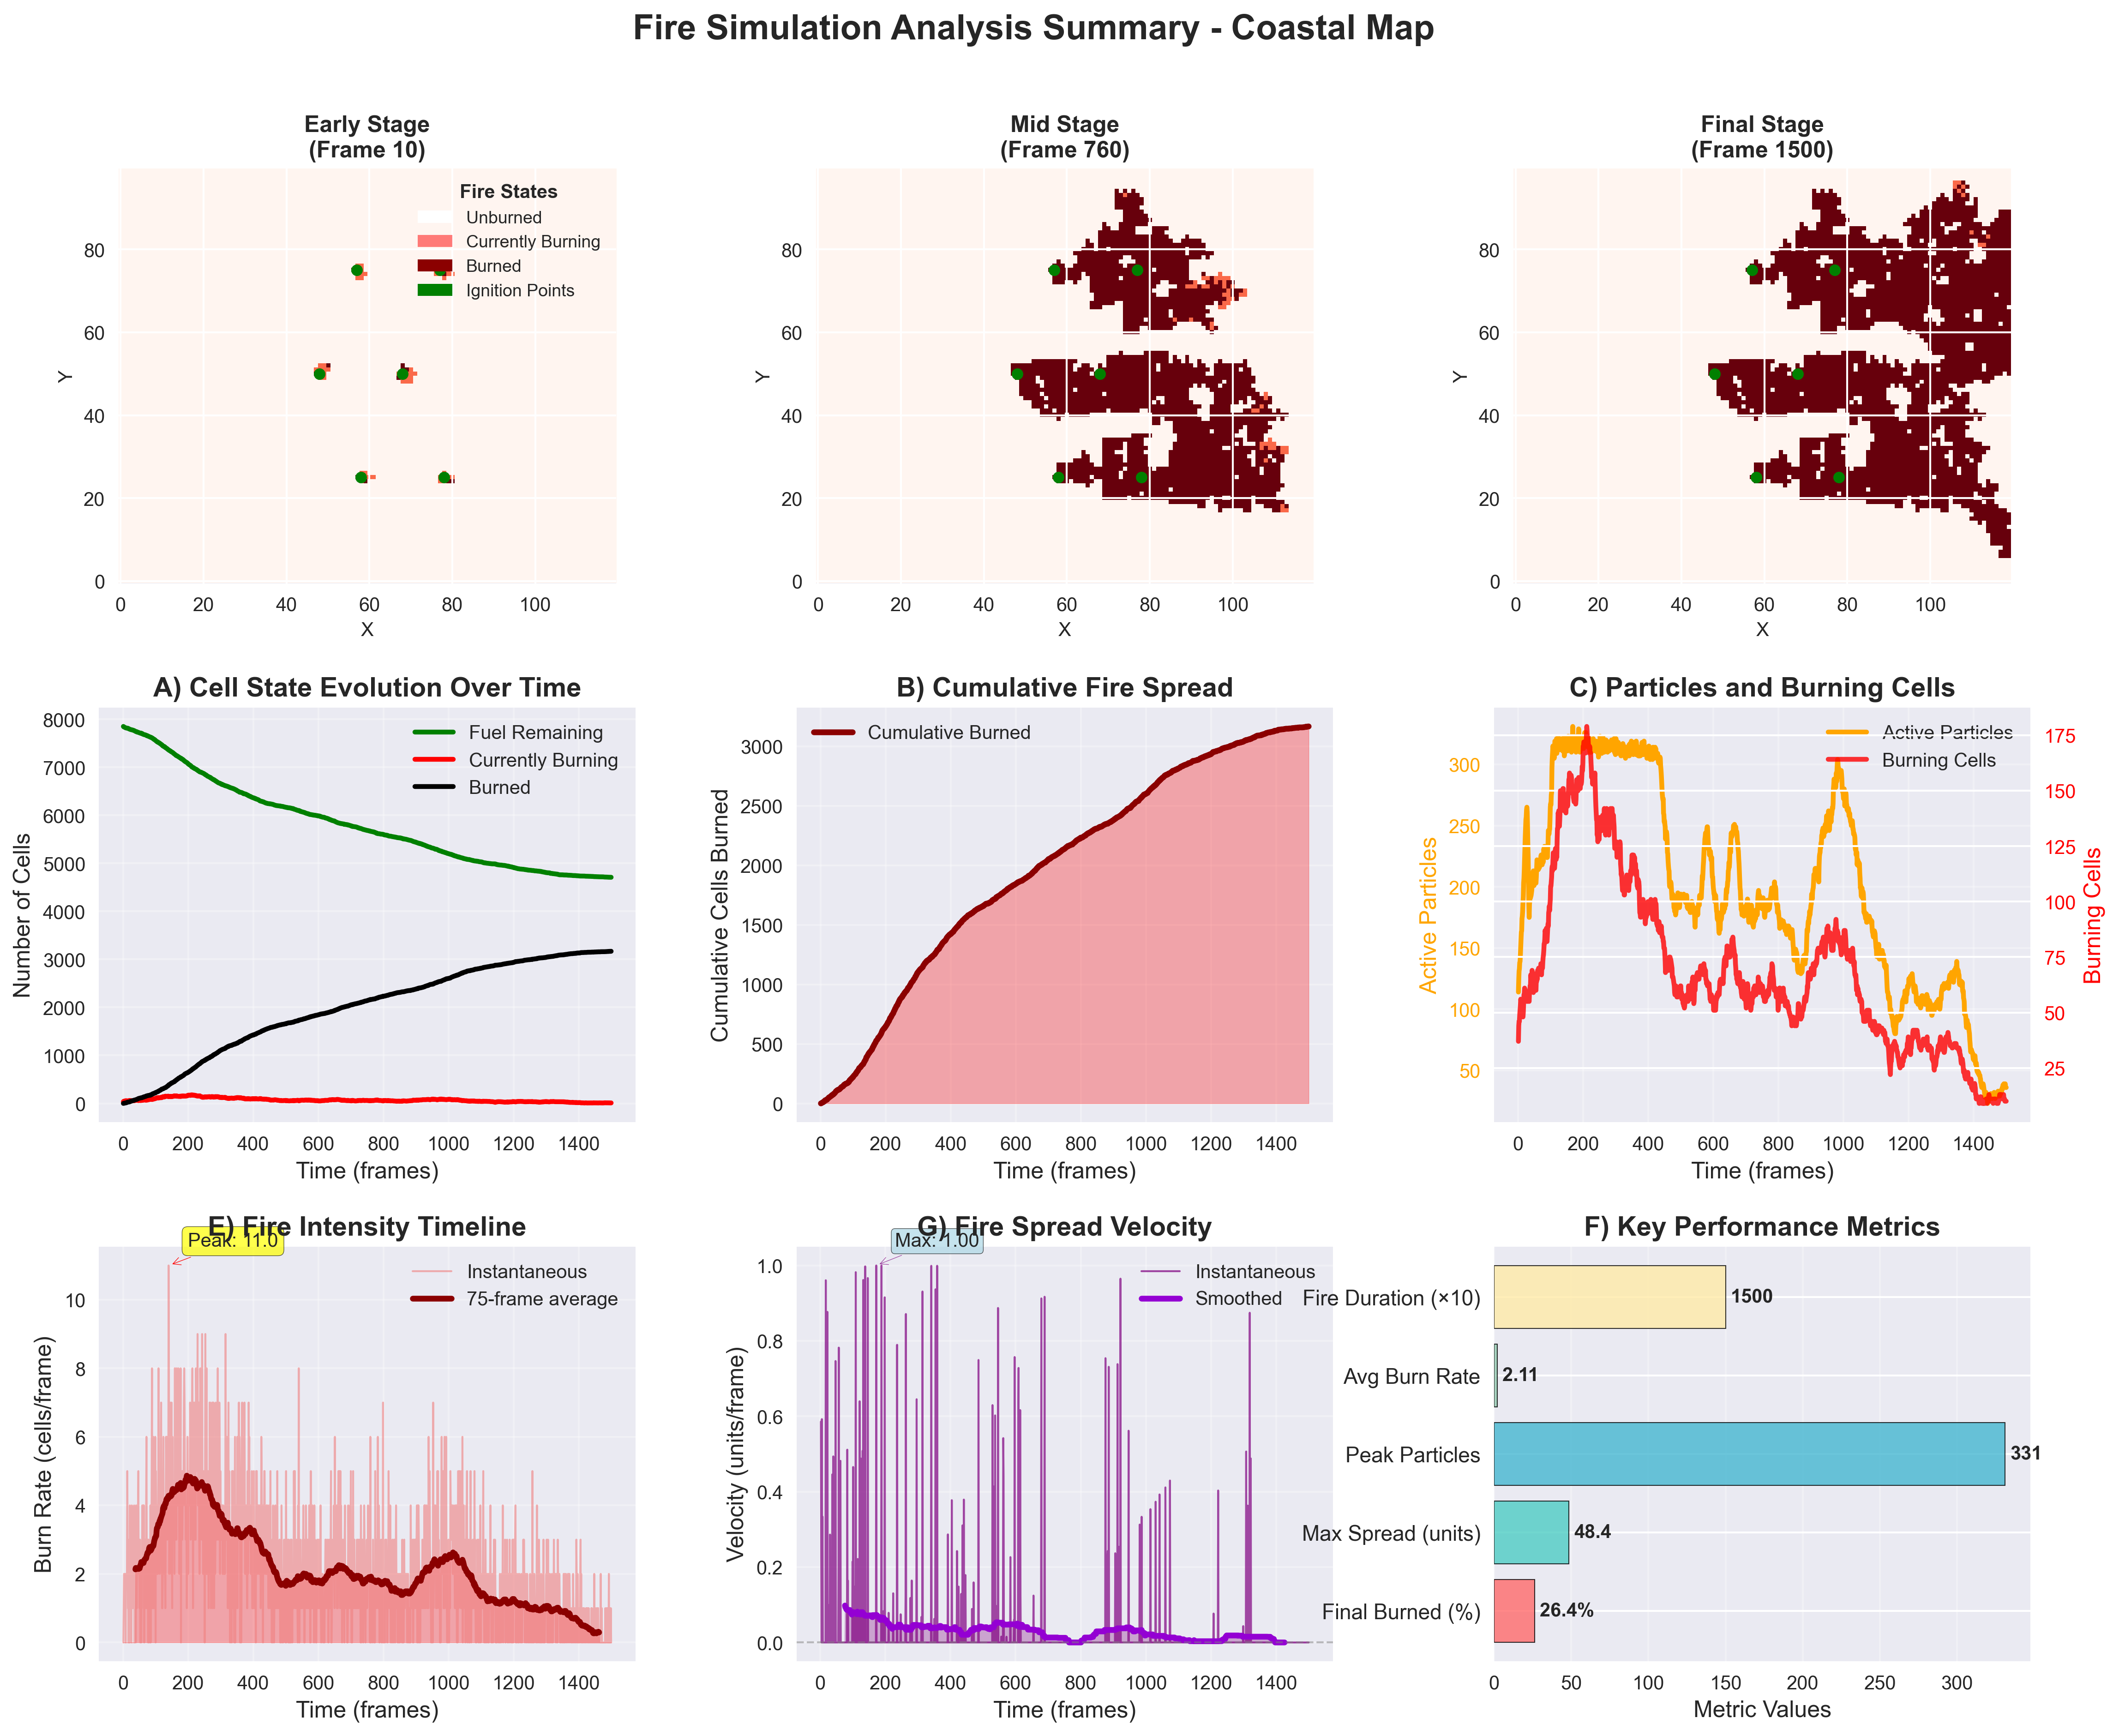
\includegraphics[width=\textwidth]{media/report_summary_coast.png}
	\caption{
		\textbf{Fire Simulation Analysis Summary - Coastal Fire Scenario.}
		Analysis of coastal fire dynamics under strong offshore wind conditions with natural moisture barriers. Top row shows fire progression from multiple coastal ignition points (left) through inland advancement (center) to final contained burn pattern (right). The analysis demonstrates the protective effect of coastal moisture gradients, resulting in 28.4\% final burned area - the lowest of all scenarios - while showing characteristic wind-driven inland fire advancement with natural coastal barriers providing effective fire suppression.
	}
	\label{fig:res_coast}
\end{figure}
